\documentclass[letterpaper]{article} % Feel free to change this
\usepackage{graphicx}
\usepackage{amsfonts}
\usepackage{amsmath}
\usepackage{amsthm}
\usepackage[utf8]{inputenc}
\usepackage[english]{babel}

\usepackage{algorithm}
\usepackage[noend]{algpseudocode}

\makeatletter
\def\BState{\State\hskip-\ALG@thistlm}
\makeatother

\newtheorem{prop}{Proposition}
\graphicspath{ {images/} }

\begin{document}

\title{ECE 590 Final Project: Scheduling with E Elevators}
\author{Hansung Kang, Kevin Kuo}
\date{\today}
\maketitle

\section{Extension to E Elevators}
\subsection{Construction}
We start by defining the sets $X_1 = \mathbb{Z}_N$ and $X_2 = \{\uparrow, \downarrow\}$. Letting $X = (X_1 \times X_2) - \{(N, \uparrow), (1, \downarrow)\}$, we can represent both the elevator position and the position of a person requesting an elevator:\\

For instance, 
\begin{itemize}
	\item If an elevator is at $(1, \uparrow) \in X$, then it is currently on the $2^{nd}$ floor ($1^{st}$ floor is at $0 \in X_1$) and moving upwards.
	\item If a person requesting an elevator is at $(4, \downarrow) \in X$, then she is on the $5^{th}$ floor and wants to move downwards. 
\end{itemize}

To make $X$ easier to visualize, we wish to arrange its elements in a circle like this:\\
\begin{figure}
  \centering
    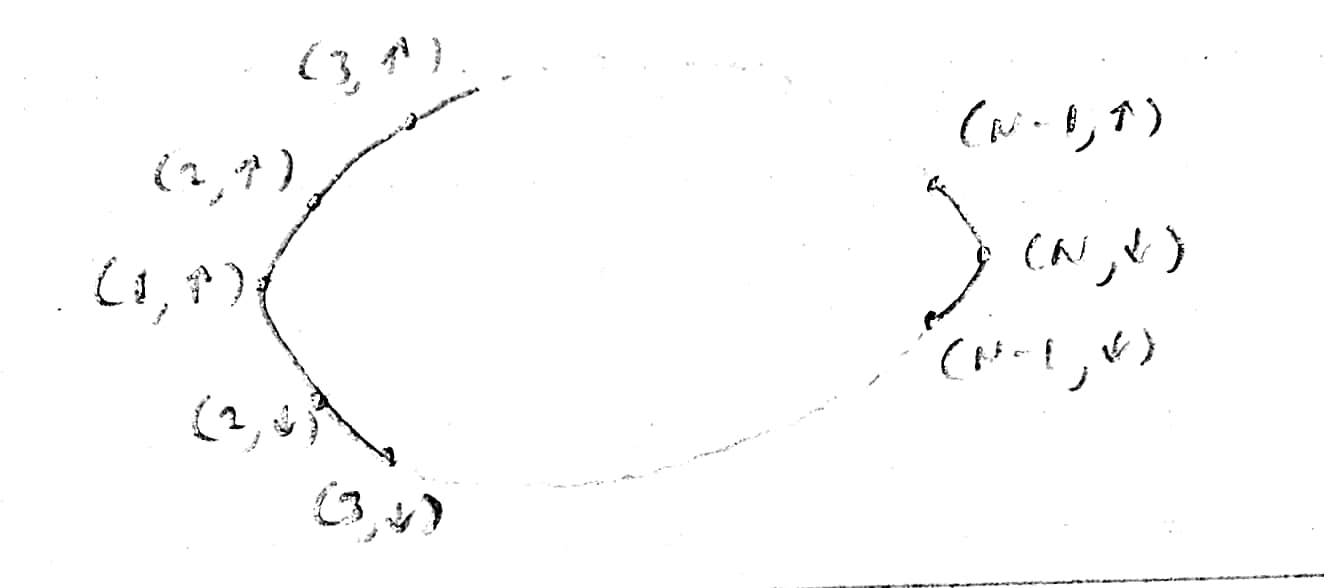
\includegraphics[scale=0.2]{circle}
  \caption{Representing $X$ as a circle}
\end{figure}
By setting the convention that elevators can only move clockwise in this circle, we can more easily visualize their paths. For instance, if an elevator wanted to move from the $3^{rd}$ floor heading up to the $2^{nd}$ floor heading down, it could travel clockwise from $(2, \uparrow)$ to $(N, \downarrow)$ to $(1, \downarrow)$. (Realistically, if the elevator did not have to stop anywhere else, it could just move straight down -- i.e. skip from $(2, \uparrow)$ to $(2, \downarrow)$, and then go to $(1, \downarrow)$. But, since the following analysis just considers the worst-case timing for the elevator (i.e. stops on every floor in between), we do not need to consider this shorter path.)\\\\
To create this circle, we map $X$ onto $\mathbb{Z}_{2N - 2}$ via $f: X \rightarrow \mathbb{Z}_{2N - 2}$ defined as \\
\begin{align*}
    f(x)=\left\{
                \begin{array}{ll}
                  \pi_{1}(x) &\text{ (if $\pi_2(x) = \uparrow$)}\\
                  (2N - 2) - \pi_{1}(x) &\text{ (if $\pi_2(x) = \downarrow$)}
                \end{array}
              \right.
\end{align*}
where $\pi_{1}(x)$ is the projection of $x$ onto $X_1$, and $\pi_{2}(x)$ is the projection of $x$ onto $X_2$. \\\\
Thus, using Figure 1 to picture $f(X)$, the top half the circle represents the values $0$ to $N - 1$ in $\mathbb{Z}_{2N - 2}$, and the bottom half represents the values $N$ to $2N - 1$.

\subsection{Worst-Case Time Analysis}
Define the map $t : X \times X \rightarrow \mathbb{Z}_N$ to be $t(x_1, x_2) = f(x_2) - f(x_1) \text{ } (mod \text{ } N)$. 

\begin{prop}
	Suppose an elevator $e \in X$ had to travel from $x_1$ to $x_2$ $(x_1, x_2 \in X)$, and the act of moving one floor and stopping took one time unit. Then $t(x_1, x_2)$ is the worst-case time it would take to make that travel. 
\end{prop}

\begin{proof}
	$e$ must travel clockwise in Figure 1. Thus, letting $T$ be the time $e$ would take, $T \leq f(x_2) - f(x_1) \text{ } (mod \text{ } N) = t(x_1, x_2)$. This upper bound is achievable if $e$ has to stop at every floor along the path from $f(x_1)$ to $f(x_2)$. 
\end{proof}

If a person waits at some point $x \in X$ with destination $d \in X$, and elevator $e \in X$ had to come to pick them up, then, by Proposition 1, the worst-case time to travel from $e$ to $x$ is $t(e, x)$, and the worst-case time to travel from $x$ to $d$ is $t(x, d)$.  Thus, the worst-case time $T$ it would take for elevator $e \in X$ to pick up the person and take them to their destination would be 
\[
	T = t(e, x) + t(x, d) 
\]
Let $\{e_1, e_2, ... , e_E\} \subset X$ be a set of elevators. Then let $T_{e_i}$ be the worst-case time defined above for elevator $e_i$. Thus 
\begin{align}
	T_{e_i} = t(e_i, x) + t(x, d)
\end{align}

\begin{prop}
	For some $i \in [1, E]$, $\left(T_{e_i} = \underset{j \in [1, E]}{\mathrm{min}} T_{e_j}\right) \Leftrightarrow \left(t(e_i, x) = \underset{j \in [1, E]}{\mathrm{min}} t(e_j, x)\right)$
\end{prop}

\begin{proof}
	If $T_{e_i} = \underset{j \in [1, E]}{\mathrm{min}} T_{e_j}$, then, by $(1)$, $t(e_i, x) = T_{e_i} - t(x, d) = \left(\underset{j \in [1, E]}{\mathrm{min}} T_{e_j} \right) - t(x, d) = \underset{j \in [1, E]}{\mathrm{min}} \left(T_{e_j} - t(x, d)\right) = \underset{j \in [1, E]}{\mathrm{min}} t(e_j, x)$.\\
	If $t(e_i, x) = \underset{j \in [1, E]}{\mathrm{min}} t(e_j, x)$, then $T_{e_i} = t(e_i, x) + t(x, d) = \left(\underset{j \in [1, E]}{\mathrm{min}} t(e_j, x)\right) + t(x, d) = \underset{j \in [1, E]}{\mathrm{min}} (t(e_j, x) + t(x, d)) = \underset{j \in [1, E]}{\mathrm{min}} T_{e_j}$
\end{proof}

\subsection{Algorithm}
Going off the previous section, to minimize the worst-case time the person at $x$ needs to wait to get to her destination, we pick the elevator $e_i$ such that $T_{e_i} = \underset{j \in [1, E]}{\mathrm{min}} T_{e_j}$. By Proposition 2, this means we choose the elevator $e_i$ such that $t(e_i, x) = \underset{j \in [1, E]}{\mathrm{min}} t(e_j, x)$. Thus, by the definition of $t$, we choose the elevator $e_i$ such that $f(x) - f(e_i) \text{ } (mod \text{ } N)$ is minimized. Note that this expression does not depend on the destination floor the person wants to go to. Thus, in a rough sense, just choosing the "closest" elevator to the person requesting one is the optimal approach to minimizing the worst-case time. \\\\
The following algorithm summarizes the approach we derived:\\\\
Let $S$ be a system of $E$ elevators $\{e_1, e_2, ... , e_E\} \subset X$. An input to $S$ would be a person represented as an element in $X$.\\
\begin{algorithm}
\caption{Minimize worst-case travel time}\label{euclid}
\begin{algorithmic}[1]
\Procedure{MinimizeWorstCaseTime}{}
\For {input $x \in X$ into $S$} 
	\State minWeight $\leftarrow \infty$
	\State minElevator $\leftarrow \emptyset$
	\For {each elevator $e \in \{e_1, e_2, ... , e_E\} \in X$}
		\State criterion $\leftarrow f(x) - f(e)$
		\If {criterion $< \text{minWeight}$}
			\State minWeight $\leftarrow$ criterion
			\State minElevator $\leftarrow e$
		\EndIf
	\EndFor
	\State add $x$ to the set of minElevator's inputs
\EndFor
\EndProcedure
\end{algorithmic}
\end{algorithm}

\subsection{A Rough Average-Time Analysis}
\begin{prop}
	Suppose that the people requesting elevators are uniformly distributed throughout the building. Also assume that their destination floors are uniformly distributed throughout the building. Then, in the long term, the elevators must also be uniformly distributed throughout the building. 
\end{prop}

\begin{proof}
	Algorithm 1 does not take into account the actual position of any person in the building -- just the relative position with respect to the elevators. Since the people requesting elevators and their destination floors are uniformly distributed throughout the building, re-numbering the building floors by adding an arbitrary integer to each floor number (modulo $N$) does not change the values calculated in Algorithm 1, and so the long-term distribution of elevators in the building is unchanged. If the elevators tended to be more focused on a specific set of floors, then the re-numbering process would cause the elevators to be focused on a different set of floors (since those floors would be re-numbered). This would contradict the fact that the elevators' long-term distribution should remain unchanged after the re-numbering, and so thus the elevators must be uniformly distributed throughout the building. 
\end{proof}

Thus, using Algorithm 1, since the elevators are uniformly distributed in the long term, a rough estimate of the average time a person requesting an elevator would have to wait is $\frac{1}{2}\frac{N}{E}$ time units. For $E = 1$, this lines up with intuition -- if a person's position is uniformly distributed, and the elevator's position is uniformly distributed, then the absolute difference between the person's and elevator's positions is uniformly distributed between $0$ and $N$, and so the person would have to wait $N/2$ time units on average. 

\subsection{Pitfalls}
In this algorithm, we do not consider the following factors:
\begin{itemize}
	\item Elevator capacity
	\item What happens when an elevator fails
	\item Time it takes an elevator to collect people at a floor
	\item The actual time it takes for an elevator to travel between floors.
\end{itemize}
We can address the first two bullet points: Step 5 of Algorithm 1 could be modified to not consider elevators that are either full or dysfunctional. \\
There are two other pitfalls to this approach:\\\\
Firstly, we only considered the worst-case time. Thus, we assumed that each elevator would stop at each floor when traversing the building. We did not do an average-time analysis, which would not make that assumption. \\\\
Secondly, we did not consider an elevator's existing stopping points. This could lead to a scenario where one elevator could be assigned a lot of people and others would not; the elevators could become unbalanced in the number of people they have to accommodate. In Algorithm 1, this can be accounted for by improving the criterion set in Step 6. For instance, the criterion could be set to $f(x) - f(e) + P_{e}(n)$, where $P_{e}(n)$ is some weighting factor dependent on the number of people $n$ currently in elevator $e$. If $P_{e}(n)$ increased monotonically with respect to $n$, then elevators that are more empty would become more likely to be chosen for the person at $x$. 

\end{document}